\documentclass[a4paper,10pt]{article}

\usepackage{graphicx}
\usepackage{geometry}
\usepackage{hyperref}
\usepackage{multirow}
\usepackage{array,makecell}

\geometry{margin=60pt,left=45pt,right=45pt}

\begin{document}\pagestyle{empty}

\noindent

\begin{tabular}{m{7cm}m{7cm}}

\multirow{2}*{\LARGE{\textbf{Petr Geršl}}} & Tel.: \textbf{+420 731 347 915} \\
& Email: \textbf{pgersl05@gmail.com}

\end{tabular}

\rule{\linewidth}{2pt}

\vspace{.4cm}

\begin{tabular}{m{7cm}m{8cm}}

\multirow{2}*{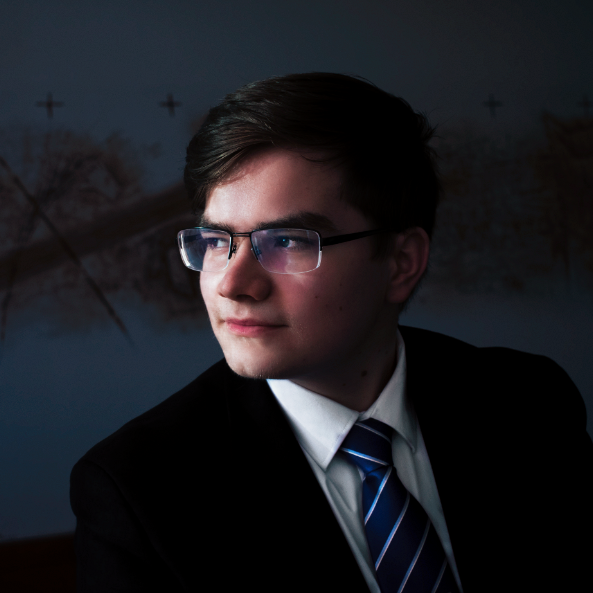
\includegraphics[width=5.4cm]{profile.png}} & Datum narození: \textbf{28. 11. 2005} \\
& Působiště: \textbf{Brno, 602 00 Brno}

\end{tabular}

\vspace{4.4cm}

\rule{\linewidth}{1pt}

\vspace{.1cm}

{\large{\textbf{Vzdělání}}}

\vspace{.7cm}

\noindent

\begin{tabular}{m{4cm}p{11cm}}

\textbf{09/2017 - doposud} & Cyrilometodějské gymnázium a střední odborná škola pedagogická Brno, gymnázium\\
\\
\textbf{09/2012 - 06/2017} & Základní škola Měnín, základní škola

\end{tabular}

\vspace{.1cm}

\rule{\linewidth}{1pt}

\vspace{.1cm}

{\large{\textbf{Zkušenosti}}}

\vspace{.7cm}

\begin{tabular}{m{1.5cm}m{3cm}p{11cm}}

\multicolumn{2}{l}{\textbf{07/2022 - doposud}} & \emph{Obchodní dům Vágner}; Česká 151/6; \textbf{prodavač} (brigáda)\\
& \textbf{reference} & vedoucí prodejny, tel. č. 731 668 617\\
& \textbf{popis činnosti} & organizace prodejny, úklid přiděleného úseku, příprava a doplňování zboží, služby zákazníkům\\
\multicolumn{2}{l}{\textbf{06/2021 - 08/2021}} & \emph{Terranova SOLITAIRE, spol. s. r. o.}; Františkánská 1 Brno; \textbf{prodavač} (brigáda)\\
& \textbf{reference} & vedoucí prodejny, tel. č. 774 996 631\\
& \textbf{popis činnosti} & organizace prodejny, úklid přiděleného úseku, příprava a doplňování zboží, služby zákazníkům\\
& \textbf{důvody odchodu} & špatné pracovní prostředí, podezřelé činnosti, nové příležitosti

\end{tabular}

\vspace{.1cm}

\rule{\linewidth}{1pt}

\vspace{.1cm}

{\large{\textbf{Dovednosti}}}

\vspace{.7cm}

\begin{tabular}{m{4cm}p{11cm}}

\multirow{2}*{\textbf{Jazykové dovednosti}} & \textbf{Čeština} (rodilý mluvčí)\\
& \textbf{Slovenština} (rodilý mluvčí)\\
& \textbf{Anglický jazyk}: (vysoce pokročilý, C2)\\ 
& \textbf{Francouzský jazyk}: (začátečník, A1/A2)\\
\\
\multirow{4}*{\textbf{Technické znalosti}} & \textbf{Kancelářské programy} (MS Office, LibreOffice, Google Workspace): středně pokročilý uživatel\\
& \textbf{Plain-text} (\LaTeX, Markdown): středně pokročilý uživatel\\
& \textbf{Web frontend} (HTML, CSS, JavaScript): středně pokročilý uživatel, vlastní projekty (\texttt{pgersl.xyz}, \texttt{astropi-hackathon.org}, \texttt{farnostmenin.cz})\\
& \textbf{Konfigurace/databáze} (TOML, JSON): začátečník\\
& \textbf{Scripting} (Python, Bash): mírně pokročilý uživatel\\
\\
\textbf{Koníčky} & studium chemie a hudební historie, hra na klavír, hudební skladba

\end{tabular}

\end{document}